%%
%% Copyright 2007, 2008, 2009 Elsevier Ltd
%%
%% This file is part of the 'Elsarticle Bundle'.
%% ---------------------------------------------
%%
%% It may be distributed under the conditions of the LaTeX Project Public
%% License, either version 1.2 of this license or (at your option) any
%% later version.  The latest version of this license is in
%%    http://www.latex-project.org/lppl.txt
%% and version 1.2 or later is part of all distributions of LaTeX
%% version 1999/12/01 or later.
%%
%% The list of all files belonging to the 'Elsarticle Bundle' is
%% given in the file `manifest.txt'.
%%

%% Template article for Elsevier's document class `elsarticle'
%% with numbered style bibliographic references
%% SP 2008/03/01
%%
%%
%%
%% $Id: elsarticle-template-num.tex 4 2009-10-24 08:22:58Z rishi $
%%
%%
%\documentclass[preprint,12pt,3p]{elsarticle}

%% Use the option review to obtain double line spacing
%%\documentclass[preprint,review,12pt]{elsarticle}

%% Use the options 1p,twocolumn; 3p; 3p,twocolumn; 5p; or 5p,twocolumn
%% for a journal layout:
%% \documentclass[final,1p,times]{elsarticle}
%% \documentclass[final,1p,times,twocolumn]{elsarticle}
%% \documentclass[final,3p,times]{elsarticle}
%% \documentclass[final,3p,times,twocolumn]{elsarticle}
%% \documentclass[final,5p,times]{elsarticle}
\documentclass[final,5p,times,twocolumn]{elsarticle}

%% if you use PostScript figures in your article
%% use the graphics package for simple commands
%% \usepackage{graphics}
%% or use the graphicx package for more complicated commands
%% \usepackage{graphicx}
%% or use the epsfig package if you prefer to use the old commands
%% \usepackage{epsfig}

%% The amssymb package provides various useful mathematical symbols
\usepackage{amssymb}
%% The amsthm package provides extended theorem environments
%% \usepackage{amsthm}

%% The lineno packages adds line numbers. Start line numbering with
%% \begin{linenumbers}, end it with \end{linenumbers}. Or switch it on
%% for the whole article with \linenumbers after \end{frontmatter}.
%% \usepackage{lineno}

%% natbib.sty is loaded by default. However, natbib options can be
%% provided with \biboptions{...} command. Following options are
%% valid:

%%   round  -  round parentheses are used (default)
%%   square -  square brackets are used   [option]
%%   curly  -  curly braces are used      {option}
%%   angle  -  angle brackets are used    <option>
%%   semicolon  -  multiple citations separated by semi-colon
%%   colon  - same as semicolon, an earlier confusion
%%   comma  -  separated by comma
%%   numbers-  selects numerical citations
%%   super  -  numerical citations as superscripts
%%   sort   -  sorts multiple citations according to order in ref. list
%%   sort&compress   -  like sort, but also compresses numerical citations
%%   compress - compresses without sorting
%%
%% \biboptions{comma,round}

% \biboptions{}

\biboptions{comma,round}


\usepackage{xspace}
\usepackage{caption}
\usepackage{xcolor}
% \usepackage[dvipsnames]{xcolor}
% % \usepackage[bookmarks=false]{hyperref}
% % \newcommand\myshade{85}
% % \colorlet{mylinkcolor}{violet}
% % \colorlet{mycitecolor}{YellowOrange}
% % \colorlet{myurlcolor}{Aquamarine}
% % \hypersetup{
% % 	linkcolor  = mylinkcolor!\myshade!black,
% % 	citecolor  = mycitecolor!\myshade!black,
% % 	urlcolor   = myurlcolor!\myshade!black,
% % 	colorlinks = true,
% % }

\usepackage{graphicx}

\graphicspath{{gfx/},{plots/}}
\DeclareGraphicsExtensions{.pdf,.jpeg,.png}
\providecommand{\norm}[1]{\lVert#1\rVert}

% *** CITATION PACKAGES ***
%



  \usepackage{mathtools}

\usepackage{amsfonts}
\usepackage{multirow}
\usepackage{rotating}
\usepackage{booktabs}
\usepackage[colorlinks]{hyperref}
\usepackage[noabbrev]{cleveref}
%\usepackage[colorlinks=true,linkcolor=black, citecolor=blue, urlcolor=blue]{hyperref}

% *** SPECIALIZED LIST PACKAGES ***
%
\usepackage{algorithm}
\usepackage{algorithmic}
\usepackage{array}
\usepackage{mdwmath}
\usepackage{mdwtab}
\usepackage{calc}
\usepackage{epstopdf}
\usepackage{listings}
\lstset{
  basicstyle=\ttfamily,
  mathescape
}




\newlength\myindent
\setlength\myindent{2em}
\newcommand\bindent{%
	\begingroup
	\setlength{\itemindent}{\myindent}
	\addtolength{\algorithmicindent}{\myindent}
}
\newcommand\eindent{\endgroup}

\newcommand{\algorithmautorefname}{Algorithm}


\journal{engineering applications of artificial intelligence}

\begin{document}

\begin{frontmatter}

\title{Oil Sands Processability Analysis Using Symbolic Regression}
%\tnotetext[label0]{This is only an example}


\author[label1,label2,label5]{Yixin Zhang\corref{cor1}}
\address[label1]{Dept. of Electrical and Computer Engineering}
\address[label2]{Dept. of Chemical and Material Engineering\fnref{label4}}

\cortext[cor1]{I am corresponding author}
%\fntext[label3]{I also want to inform about\ldots}
%\fntext[label4]{Small city}

\ead{yixin6@ualberta.ca}
%\ead[url]{author-one-homepage.com}

\author[label1,label5]{Qing Zhao}
\address[label5]{University of Alberta}
\ead{qingz@ualberta.ca}

\author[label2,label5]{Zhenghe Xu}
\ead{zhenghe@ualberta.ca}




\begin{abstract}
Hot or warm water based bitumen production process from mineable oil sands is extremely complex in nature and highly sensitive to variability of oil sands ores and process conditions. Understanding ore processability and developing sensible markers for ore processability are considered to be a challenging task. In addition to processing variables such as temperature, hydrodynamics, process water chemistry and chemical additives, ore characteristics, such as bitumen content, connate water content and chemistry, fines content and more importantly types of fines play a decisive role in determining the processability of oil sands ores. It is therefore valuable to analyze the processability of oil sands ore using statistical modelling approaches. In this paper, a symbolic regression method based on genetic programming is applied to understanding oil sands ore processability, such as identifying sensible markers of ore processability. The analysis is conducted using variety input variables representing ore characteristics and operating conditions. The model is expressed analytically by a combination of these input variables and a given set of math operators and constants. This model provides a reliable prediction for the response variables, e.g, bitumen recovery. The results show an agreement between simulation and experiment data, highlighting the applicability of the Symbolic Regression (SR) method in identifying a mathematical model to describe the mechanisms involved in oil sands processing. 
\end{abstract}

\begin{keyword}
%% keywords here, in the form: keyword \sep keyword
Symbolic Regression, Genetic Algorithm, Genetic Programming, Kernel Methods, Oil Sands Processability, System Identification
%% MSC codes here, in the form: \MSC code \sep code
%% or \MSC[2008] code \sep code (2000 is the default)
\end{keyword}

\end{frontmatter}

%%
%% Start line numbering here if you want
%%
% \linenumbers

%% main text
\section{Introduction}
\label{sec1}

A significant portion of bitumen produced in Canada is from the mineable oil sands \cite{masliyah2004understanding}. Hot water based bitumen production process from mineable oil sands is extremely complex in nature and highly sensitive to variability of oil sands ores. Understanding ore properties and developing a sensible marker for ore processability have been proven to be highly desirable but challenging. Not only process variables but also ore characteristics play a decisive role in determining the processability of oil sands ores. There are three main contributing factors for poor performance of oil sands extraction\cite{Fong2004}: \emph{(1)} lack of on-line determination of complex oil sands composition; \emph{(2)} lack of advanced setup for process control; and \emph{(3)} malfunctions or failures of mechanical equipment.

The current technology for improving oil sands processability is mostly based on single factor analysis or factorial design, which has not yielded satisfactory results. In recent years there have been considerable efforts and extensive development of machine learning and data driven techniques for process modeling and analysis. It is expected that these emerging techniques and knowledge will provide new means for tackling challenging tasks of oil sands process analysis. Using plant or Batch Extraction Unit (BEU) data, algorithms based on probabilistic programming and/or statistical data analysis have recently been applied to modeling oil sands ore processing\cite{zhang2004artificial}.

Recently, machine learning methodology has initiated lots of academic and industry attempts in the field of engineering application. There are various research developments such as using evolutionary method finding re-entry vehicle path \cite{sushnigdha2017evolutionary}. In planning and manufacturing process, machine learning application are also widely used for building feature beasd design of computer aided process planning intelligent system \cite{kumar2017state}. Researchers nowadays can even use evolutionary methodology to track a moving object using robot system \cite{sangdani2018genetic}. In machine learning field, evolution computing is a very specific subject and genetic algorithm (GA) can represent its essence.


Genetic Algorithm is a unique and useful family of techniques in data analysis. In recent years, there has been a significant amount of research on genetic algorithm that focuses on particular characteristics of data and whereat factors and their associations. Symbolic Regression (SR), for example, focuses on identification of a mathematical description on a hidden system from experimental data. The applications of SR algorithms have grown significantly during the past years. It has been shown that they could be a successful solution to dimensionality reduction modelling and optimization in a variety of areas including but not limited to environmetrics \cite{gen2000genetic}, microarray data analysis [5-7] %\cite{brunet2004metagenes,devarajan2008nonnegative,KozaGP}%, 
document clustering \cite{berry2005email}, face recognition [9-11]%\cite{BurkardtImageGA, zafeiriou2006exploiting,kotsia2007novel}%
, blind audio source separation \cite{weninger2012optimization} and more. What makes SR algorithms particularly attractive is the function constraints imposed on the factors they produce, allowing for better interpretability. 


\textcolor{red}{(remove and instead, explain how blockers are introduced and can self-evolve?)}



In this work, the main objective is to identify significant markers for processability of mineable oil sands ores, based on which prediction results can be produced, which will potentially be integrated with the current industrial analysis system. In our approach, several sensible markers controlling the ore processability are identified, and analytical relationship between these markers and the oil recovery are to be established.

A preliminary SR  framework for genetic algorithm suitable for prediction of oil sands ore processability analysis was proposed as shown in \autoref{fig:GP_procedure.png}. A greedy genetic algorithm is adopted   to optimize the factors of the oil sands recovery prediction. The statistical mathematical characterization results are then obtained by SR. In order to extract features that are more meaningful, a modification to the SR algorithm is considered which incorporates certain partially known information/constraints of the input attributes of given dataset. In this paper, SR algorithm is applied not only to simulated data (mainly for proof of concepts and verification), but also to the plant data for further validation and demonstration of the applicability. 

% \undeline{In the rest of the paper, Section 2 explains the methodology of SR, Section 3 presents the genetic programming procedure used for SR, Section 4 gives an experimental dataset used in the study, Section 5 presents another real world dataset. Section 6 concludes the paper.} (this an be removed)  



\section{Methodology}

\subsection{Symbolic Regression via Genetic Programming}  


In this paper, the symbolic regression (SR) via genetic programming (GP) is applied to analyzing oil sands processability. 
A genetic programming is an optimization procedure. From a given population $X$, it seeks item $x \in X$, which has the greatest fitness. A genetic programming searches for the best value by creating a small pool of random candidates, selecting the best candidates, allowing them to breed with minor variations, and finally repeating this process over many generations. These ideas are all inspired by the analogy to the evolution of living organisms\cite{gen2000genetic}.


\begin{figure}[!htbp]
	\centering
	\includegraphics[width=0.3\textwidth]{B.png}
	\vspace{-2em}
	\caption{Genetic Programming(GP) iteration procedure: The tree-based GP iteration controls the evolved SR generation and destruct the unpromising offspring.}
	\label{fig:GP_procedure.png}
\end{figure}

A genetic programming typically includes:

\begin{itemize}
	\item{a genetic representation of candidates;}
	\item{a way to create an initial population of candidates;}
	\item{a function measuring the fitness of each candidate;}
	\item{a generation step in which some candidates die, some survive and others reproduce by breeding;}
	\item{a mechanism that recombines genes from breeding pairs and mutates others.}
\end{itemize}



Symbolic regression (SR) is a method to search for a set of mathematical operators that identify an analytical description for the relationships among input and output attributes of the given data set. SR aims to extract an appropriate model from a space of all possible expressions $\mathcal{S}$ defined by a set of given binary operations (e.g., $+$, $-$, $\times$, $\div$, etc.) and mathematical functions (e.g., $\sin$, $\cos$, $\exp$, $\ln$, etc.), which can be described in the following nonlinear optimization problem:
\begin{equation}
\label{SRdef}
f^*=\arg\min_{f \in \mathcal{S}}\sum_i\left\|{f(\mathbf{x}^{(i)})-y_i}\right\|,
\end{equation}
where $\mathbf{x}^{(i)}\in{\mathbb{R}^d}$ and $y_i\in{\mathbb{R}}$ are input observations and output data, respectively. $f$ is the unknown target model and $f^*$ is the identified data model. SR is an NP-hard problem that can be solved using genetic algorithm. Moreover, a standard algorithm used for SR is GP, which is specialized for evolving generation and tree structures, e.g, searching for a space of mathematical expressions and minimizing various error metrics. Both the parameters and the form of equations are subject to search. In SR, many initial random symbolic equations compete via optimization to model experimental data in a most non-traditional manner. New equations are formed by reorganizing and combining previous equations and probabilistically varying their sub-expressions. The algorithm leads to equations that model the experimental data and at the same time the rejection of unpromising solutions.  After an equation reaches a desired level of accuracy, the algorithm terminates, returning equations that may correspond to the intrinsic mechanisms of the original dataset\cite{schmidt2009distilling}. The overall procedure summarizing the above steps is shown in \autoref{fig:GP_procedure.png}.

In SR, the representative symbolic expressions are the combination of genes often represented as a binary tree of algebraic operations with numerical constants and symbolic variables as its leaves. Other more complex representations include acyclic graphs and grammars \cite{tsoumakas2007multi}. The fitness of a particular equation is a numerical measure of how well it agrees with the data, such as the correlation of equation-generated results and the experimental data.

The expressions can vary among many mathematical operators, including \textit{abs}, \textit{exp} and \textit{log} etc., or binary ones such as \textit{add, sub, multiply}, and \textit{divide}. If prior knowledge of the initial value is known, which is the so-called domain knowledge, the types of operations available can be chosen ahead of time. The terminal values consist of constants, and input attributes or function variables.

Mutation in a symbolic expression can change an operator in the binary tree, e.g, it can change the \textit{add} functions into \textit{sub}, change the arguments of an operation such as changing $x+c$ to $ x+x$, delete an operation such as changing $x+x$ to $ x$ or add an operation by changing $x+x$ to $ x+(x+x)$. If the operator is changed from a binary operation to a constant, one of the two sub-tree branches is discarded and those branches can be chosen randomly.

Crossover of a symbolic expression exchanges sub-trees in the binary trees of the initial expressions.  For example, crossing $f(x) = x^2+c$ and $f(x) = x^2 + sin(x) +x$ could produce a sub tree with $f(x) = x^2+sin(x)$, from which the leaf node $c$ was exchanged with the $sin(x)$ term.

\subsection{SR Parameters and Constrained Optimization} 
 
In SR, once the fitness function is defined constrained optimization {\color{red} (with obtained symbolic expressions as the constraints)} should be performed by treating every constant as the parameter. The constrained optimization can also be treated as a fitting problem by minimizing a cost function $Q(\alpha)$ (\autoref{eq:optimization_function}), which can be chosen the sum of squared errors between the experimental data $y$ and the prediction of the SR expression $f(x,\alpha)$. Such optimization can be evaluated by using algorithmic differentiation, also called automatic differentiation (AD) \cite{neidinger2010introduction}. AD is a useful tool in practical optimization problems involving calculation of first or high-order derivatives of the objective or constraint functions that are given in computer programs. 

\begin{equation} \label{eq:optimization_function}
Q(\alpha) = \sum_{i=0}^{m}(y_i-f(x_i,\alpha))^2
\end{equation}
where $x_i$ is input variable and $\alpha$ is model parameter.


One of the conditions for SR to work is that differentiable (smooth) functions such as logistic functions must be incorporated in the SR parsing tree, which encodes formula expression using combination of the identified markers. Otherwise optimization solutions with one or multiple sets cannot be achieved by the gradient calculation. The gradient of this SR model can generate a continuous search direction, whose information can be used for accelerating this entire process.

The constrained optimization is an iterative procedure which gradually improves the SR model quality using the gradient calculation, starting from initial parameters. As a start, the Jacobian matrices are evaluated, which are used to update the parameter vector for the iteration procedure to continue until a specified stopping criterion is reached. automatic differentiation is used for the calculation of all partial derivatives with respect to the parameter vector $\alpha$. As a result, all constant values are extracted and replaced by an appropriate parameter $\alpha_i$, given in \autoref{eq:function_derivative},

\begin{equation} \label{eq:function_derivative}
\nabla f = \left( \frac{\partial f}{\partial \alpha_1},
\frac{\partial f}{\partial \alpha_2}...
\frac{\partial f}{\partial \alpha_i}\right)
\end{equation}



% \begin{figure}[!hptb]
% 	\centering
% 	\includegraphics[width=\linewidth,clip]{learning_path.png}
% 	\vspace{-2em}
% 	\caption{The
% 		execution of the first individual (covering the six nodes 1,
% 		3, 4, 5, 7 and 8 on the target path) will lead to a high
% 		approximation level if all identical path sections are
% 		considered for the fitness evaluation. If only the first
% 		matching path section is measured, the second individual
% 		(covering five nodes 1, 2, 3, 4 and 7) will lead to a higher
% 		approximation level than the first one\cite{baresel2002fitness}}.
% 	\label{fig:learning_path.png}
% \end{figure}

\begin{figure*}[!htbp]
	\begin{center}
		\captionsetup{labelformat=empty}
		\caption*{Table 1. Comparison of SR with three other modeling techniques (Linear Regression, Neural Networks and Random Forests) which belong to three distinct culture in modeling prediction family \cite{vladislavleva2010knowledge}.}.
		
		\includegraphics[width=\linewidth]{SR_comparison.png}
	\end{center}
	\label{Table:SR_comparison}
\end{figure*}

{\color{red}(the following paragraph together with Figure 2 need to be rewritten for better explanation)}

% In addition, artificial nodes are introduced in the SR model to include nonlinear scaling terms. In one iteration, the start values for the SR model are the previously extracted constraint values in terms of additive and multiplicative scaling terms. The length of all path sections is unknown but is assumed to be a fixed value as approximation. Because a high fitness value can be achieved by covering the desired path to the convergence criterion from the initial start target, the combination of two such nodes may lead to considerably better offsprings. The procedure is shown in \autoref{fig:learning_path.png}. The algorithm is stopped after a customized number of iterations. Individual parameters for optimized constants would be updated. Meanwhile, the optimization starts from the same values which are automatically retrieved in the model. This procedure is repeated many times by tuning the parameter vectors until a stopping criterion is met.
The designed algorithm describing necessary steps for the proposed SR-based model is given as \autoref{algo:deepnmfalgo}. In the literature, the SR method has been utilized in many application areas. SR is able to understand the data and build a descriptive model. Most importantly it provides certain insights about the data and the model. Table 1 provides comparison among several data mining methods, including SR. In section 3, we demonstrate the application of SR to the analysis of oil sands ore properties. 


\begin{algorithm}[!htbp]
	\caption{This proposed algorithm for training a SR model: Initially we approximate the factors greedily using the automatic differentiation algorithm \cite{neidinger2010introduction} and then fine-tune the factors until the convergence criterion is satisfied.}
	\label{algo:deepnmfalgo}
	\begin{algorithmic}
		
		\STATE {\bfseries begin:}
		\STATE {}
		\bindent
		\STATE {Set the generation counter to 0; and randomly initialize a population of individuals $x_i$}. 
		\STATE {}
		\STATE {Initialize the tuning parameter $\alpha$. Set up the initial searching function.}
		\STATE {}
		\STATE {Evaluate the fitness value for each individual in each iteration.}
		\STATE {}
		\eindent
		\WHILE {stopping criteria are not satisfied}
		\STATE {}
		\STATE 	{\bfseries for} {i=1} to population size {\bfseries do} 
		
		
		\bindent
		\STATE		{	start with selected initial searching function}
		%\eindent
		
		\bindent
		\STATE 	{\bfseries for} {j=1} to randomly chosen index {\bfseries do}
		\eindent
		\STATE {}
		\bindent
		\STATE  {Mutation: generate a mutant individual using automatic differentiation strategy}
		\STATE {}
		\STATE	{Crossover: mix mutant individual and feasible individual to generate a trial offspring $\hat{x}_j$}
		\eindent
		%\STATE		{$J_{rand}$=[rand(0,1)*index]}
		\STATE {}
		
		%\STATE 	{\bfseries for} {i=1} to population size {\bfseries do}
		\bindent
		\STATE {evaluate the fitness value of offspring $\hat{x}_j$}
		\eindent
		\bindent
		\IF {$\hat{x}_j$ is better than $x_i$}
		\STATE {$x_i$ = $\hat{x}_j$}
		\ENDIF
		\eindent
        \STATE 	{\bfseries end for}
        \eindent
        \STATE 	{\bfseries end for}
		
		\ENDWHILE
		
		
	\end{algorithmic}
\end{algorithm}


\section{Implementation Procedure}\label{sec:experiments}
In this section, details on how to implement the SR-based algorithm are given first, and then as an example the algorithm is applied to a set of synthetic data which is generated to mimic the oil sands recovery process in a laboratory experiment. 
\subsection{Problem Setup}

To implement the SR-based genetic programming, the following steps are needed:
\begin{enumerate}
	\item  Binary representation conversion. 
	%\vskip 0.1in
	\item  Initial population setup.
	%\vskip 0.1in
	\item  Fitness measurement.
	%\vskip 0.1in
	\item  Death, breeding, and mutation.
\end{enumerate}

For this study, we choose six decimal digits of accuracy to create the possible solutions when converting the dataset using binary representations in step 1. Six decimal digits of accuracy corresponds to about 22 binary digits. A 22-digit binary string $b$ can be converted
to an integer $k$ which is given by:
\begin{equation}
k = \sum_{i=1}^{22} b_i \cdot 2^{i-1}
\end{equation}
The integer $k$ is then converted to a real number $u$ between 0 and 1 by:
\begin{equation}	
u = k / ( 2^{22}-1)
\end{equation}
The number $u$ is then converted to a real number $r$ between -1 and +2 by:
\begin{equation}	
r = -1 + 3 \cdot u
\end{equation}
with these procedures, we have a mapping between genetic information $b$ and
the objective $r$.

\subsection{Implementation Details}

This section is mainly focused on demonstration of SR procedure, and for simplicity, during the modeling process, only a single input variable temperature (T) from the synthetic oil sands data is selected and the SR model output is the recovery rate (R). The complete simulation and analysis results considering more input variables will be described in detail in Section 4. 


Each variable is initially given a string of 22 binary digits, which can be treated as an integer vector.
\vskip 0.1in
Choosing a population of $n = 50$ candidates, we create a 2 dimensional array of size $50 \times 22$.
\vskip 0.1in
A random initial population corresponding to $T$, which can be selected as an array of 0's and 1's, is given below as an example.

\begin{lstlisting}


i  ----------b-----------     ----converted value of T----   
#1  1000101110110101000111  =             0.637197               
#2  0000001110000000010000  =             -0.958973              
...
#50 1110000000111111000101  =             1.627888               
\end{lstlisting}
The best individual is searched for the optimized output quantity $R(T)$.
\vskip 0.1in
In this study, the initial searching function is chosen as follows:
\begin{equation}	
R(T) = T \cdot \sin ( 10 \pi \cdot T ) + 1
\end{equation}

Based on this initial selection, the iteration begins by evaluating the fitness of each candidate as follows:
\begin{lstlisting}
i  -----------b----------  converted value of R(T)        $Q(\alpha)$
#1  1000101110110101000111      1.586345               0.097567
#2  0000001110000000010000      0.078878               0.124862
...
#50 1110000000111111000101      2.250650               0.067429
\end{lstlisting}	



Based on the fitness results, the following steps are performed for the next
iteration:
\begin{itemize}
	\item {Out of the 50 candidates, remove 10 candidates with the lowest fitness; }
	\item {Let the 10 candidates with the highest fitness breed in pairs, creating 10 new candidates;}
	\item {Randomly select 2 of the nonbreeding, nondying candidates for mutation;}
\end{itemize}
\vskip 0.1in
The size of the new population remains unchanged when it contains the best candidates from the previous population. The 10 candidates with lower score are replaced by new offspring of higher fitness score. For the intermediate 30 candidates, we modify two candidates randomly by mutation and keep 28 candidates unchanged.
\vskip 0.1in
For mutation, a candidate $i$ can be picked to mutate. It is known that each candidate
has 22 bits of genetic information. For example, one can pick index $j$ between 1 and 22 and
flip that bit:

\begin{lstlisting}
b(i,j) = 1 - b(i,j)
\end{lstlisting}
\vskip 0.1in
For breeding, we assume parents $i_1$ and $i_2$ creating children $i_3$ and $i_4$.
To achieve this, an index $j$ between 1 and 21 is chosen and parental information can then be spliced together as follows:
\begin{lstlisting}
b(i3,1:j) = b(i1,1:j)& b(i3,j+1:22)
b(i4,1:j) = b(i2,1:j)& b(i4,j+1:22)
\end{lstlisting}

Given the candidate \#50 which is:
\begin{lstlisting}
i  -----------b---------- converted value of R(T)

#50 1110000000111111000101     2.250650
\end{lstlisting}
If the fifth gene in this candidate is mutated, then the result is
\begin{lstlisting}
1110100000111111000101  =>  -0.082257 => $Q(\alpha)$ = 0.736912
\end{lstlisting}
but if the 10th gene is mutated, then the following result is obtained:
\begin{lstlisting}
1110000001111111000101  =>  2.343555  => $Q(\alpha)$ = 0.065371
\end{lstlisting}
Thus, a mutation process can be controlled to improve the fitness value.

The following shows the results of breeding. For example, we make candidates \#2 and \#50 breed, 
\begin{lstlisting}
i  -----------b---------- converted value of R(T)   $Q(\alpha)$
#2  0000001110000000010000       0.078878         0.124862
#50 1110000000111111000101       2.250650         0.067429
\end{lstlisting}
The crossover point is defined as a selection of parental information to generate offspring. 
If the crossover point is after $j=5$, the two children will be as follows. 
\begin{lstlisting}
-----------b---------- converted value of R(T)    $Q(\alpha)$
0000000000111111000101       0.940865           0.187592
1110001110000000010000       2.459245           0.078346
\end{lstlisting}
It is obvious that one child has a significant increase in the fitness function.

The GP procedure is terminated after 441 iterations. For the simulated data, intermediate results from the symbolic regression algorithm in several steps are shown in Table 2. The final results and the performance validation are included in Section 4. 

\begin{table}[!hptb]\label{tab:iteration}
	\begin{center}
		\captionsetup{labelformat=empty}
		
		\caption{Table 2. Results of SR descriptor via genetic programming for a single input variable T.}
		
		\begin{tabular}{|r|l|}
			\hline
			Iteration & $R(T)$ \\
			\hline
			1 & $T \cdot \sin ( 10 \pi \cdot T ) + 1$ \\
			6 & $T$ \\
			8 & $16.2+T$ \\
			9 & $34.3+1.08 \cdot T$ \\
			10 & $61.7+29\sin(4.14+0.0519 \cdot T)$ \\
			12 & $61.7+43.9\sin(4.23+0.0517 \cdot T)$ \\
			39 & $18.3+73 \cdot logistic(0.465 \cdot T-16.6)$ \\
			40 & ... \\
			51 & ... \\
			99 & $18.2+0.000165 \cdot T^2 +72.3 \cdot logistic(0.468 \cdot T-16.7)$ \\
			120 & ... \\
			441 & $9.7 + 0.00025 \cdot T^3 + 3.75 \cdot T \cdot logistic(0.58 \cdot T - 18.39)$ \\ 
			& $- 0.054 \cdot T^2 \cdot logistic(0.58 \cdot T - 18.39)$ \\
			\hline
		\end{tabular}
		
	\end{center}
\end{table}

\section{Results of SR Descriptor using Simulation and Laboratory Data} \label{sec:related}

The oil sands data set contains three input variables: Temperature (T), pH, and Clay fines (Cf). The output is oil sands processability index, bitumen recovery (R). Due to lack of industrial data, we use data from laboratory experiments together with the generated simulation data. The simulation data set contains 1000 data points, which are generated based on known and empirical knowledge about relations among variables. Furthermore, it is noted that symbolic regression requires repeated simulation from multiple data generation. This can be achieved by adding noises and changing noise profiles to repeat the simulation.

Applying the SR to the simulated oil sands dataset led to a descriptor (i.e. a mathematical expression) for the factor analysis of bitumen recovery after 742 iterations. 
In this section, we will construct and evaluate the performance of the descriptor by calculating the mean square error between the original data and reconstructed data for all input variables. In order to have comparable results, all of the temporary descriptor are set to the same termination criterion. We have set the maximum amount of iterations to 1000. As explained in Section 3, the final descriptor obtained by the SR for all three inputs is shown in \autoref{eq:deep_nmf_linear_cost}, which presents several sensible markers and their relationships constructed from the data used in this study. 


\begin{align} \label{eq:deep_nmf_linear_cost}
\notag    R &=  0.39 \cdot T \cdot pH + 25.5 \cdot logistic(0.0597 \cdot pH)\\\notag 
%\notag   R = 0.39 \cdot T \cdot pH + 25.5 \cdot logistic(0.0597 \cdot pH)\\\notag
&\qquad + 0.00783 \cdot pH^2 \cdot Cf^{-3} + 5.79 \cdot logistic(0.001 \cdot pH^3)\\\notag 
&\qquad +0.049 \cdot T^2 -0.035 \cdot T^3-0.002\cdot T \cdot pH \cdot Cf^{-2}\\\notag 
&\qquad + 0.00369 \cdot Cf^{-4} \cdot logistic(0.001 \cdot Cf^{-3})\\\notag
&\qquad +...\\
\end{align}
It should be noted that the terms shown in \autoref{eq:deep_nmf_linear_cost} are considered to be the key factors that can describe most of the relationship (higher coverage), and ... represents the other terms of lower importance that can be ignored due to lower coverage.

The SR descriptor shows a clear representation of the simulation data, which demonstrates characteristic features of input attributes. Such a descriptor can also be improved by integrating physical insights as constraints, such as function candidate blockers or generators during SR iterations.
 
\autoref{fig:T_SR} shows the descriptor's output (i.e. the approximated recovery rate) with respect to temperature, in comparison with the training data ($\circ$). The training dataset contains a mixture of real laboratory data and the simulation data, since the few number of laboratory data alone do not contain enough information to describe the bitumen recovery. It is clear that result in \autoref{fig:T_SR} shows an excellent description of recovery dependence on temperature in \autoref{eq:deep_nmf_linear_cost}.


\begin{figure}[!hptb]
	\centering
	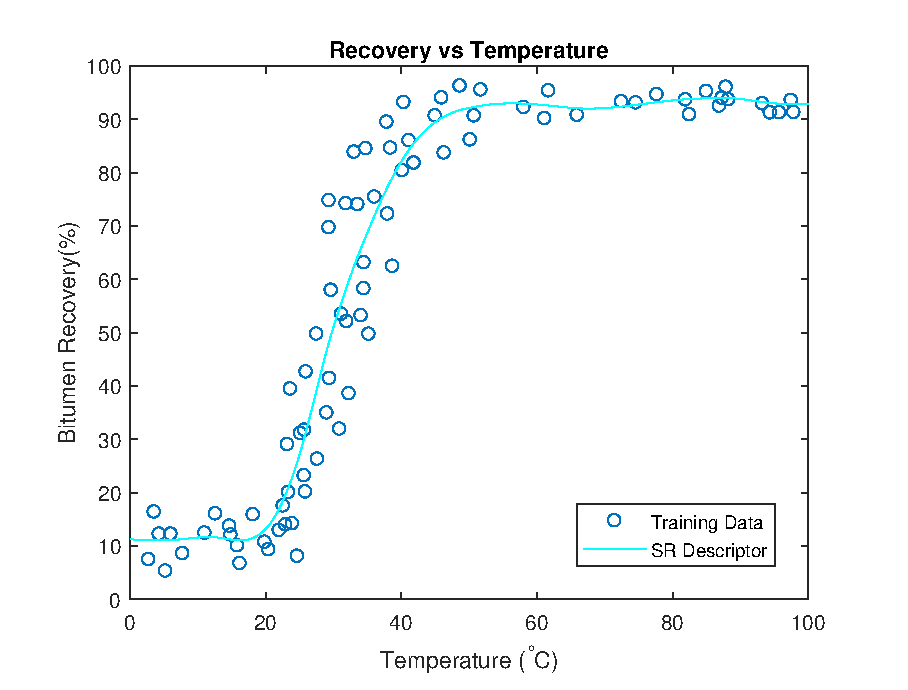
\includegraphics[width=\linewidth,clip]{T_SR.eps}
	\vspace{-2em}
	\caption{Symbolic regression prediction of the relationship between bitumen recovery and temperature.}
	\label{fig:T_SR}
\end{figure}





\begin{figure}[!hptb]
	\centering
	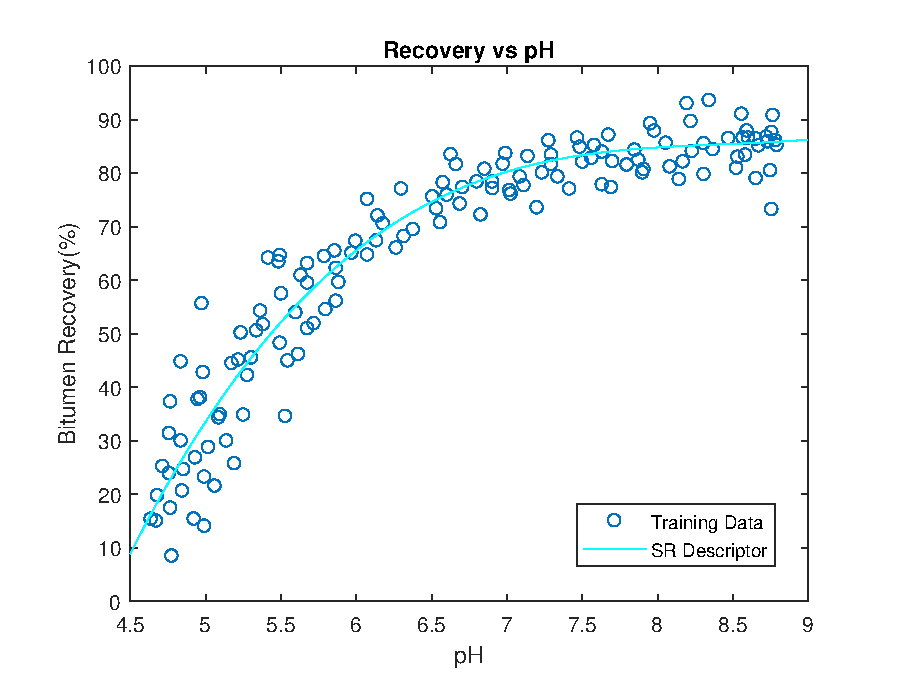
\includegraphics[width=\linewidth,clip]{pH_SR.eps}
	\vspace{-2em}
	\caption{Symbolic regression prediction of the relationship between recovery and pH.}
	\label{fig:pH_SR}
\end{figure}


\begin{figure}[!hptb]
	\centering
	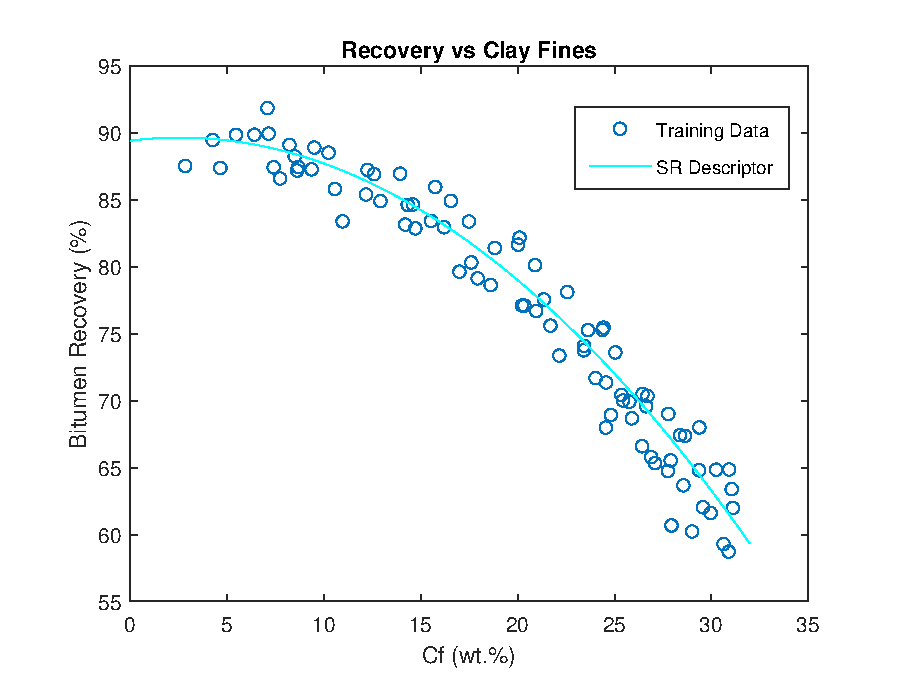
\includegraphics[width=\linewidth,clip]{CF_SR.eps}
	\vspace{-2em}
	\caption{Symbolic regression prediction of the relationship between recovery and Cf.}
	\label{fig:CF_SR}
\end{figure}


\autoref{fig:pH_SR} shows clearly how the bitumen recovery varies with slurry pH: starting from 10\%  at pH 4.5 with a rapid increase as pH increases to 7, followed by a slower increase to reach around 85\%  at pH 9.0. The results in \autoref{fig:CF_SR} show an opposite trend of decreasing biutmen recovery with increasing clays content.

Note that the descriptor found strongly depends on the selection of objective or fitness function. In this study, we simply select $Q(\alpha)$ (\autoref{eq:optimization_function}) as the measure of the error when fitting the descriptor with the given input-output data. However, more selections can be tested such as stochastic universal sampling, or the tournament selection method \cite{whitley1994genetic,blickle1995mathematical}.
%Thus, the SR descriptor from the simulation data set has richer interpolation in features domain. Counter-intuitively, the descriptor from this oil-sands artificial dataset becomes more reliable by changing parameter $\alpha_i$ in Equation 2. Despite that, we can use $\alpha_i$ to influence the shape of the SR curve. Overall the most accurate model of the data set is still the most accurate model.


To assess the quality and accuracy of the descriptor, comparison of the predicted results from the descriptor and the original laboratory data is performed in \Cref{t_comparison,ph_comparison,Cf_comparison}. \autoref{t_comparison} shows the constructed relationship of the bitumen recovery with respect to the temperature, with comparison to the original laboratory data used in the dataset. By increasing the clay fines from 20 wt\% to 30 wt\%, two different curves are generated by SR descriptor which share the similar trend showing how the bitumen recovery is affected by temperature from 10 to 90 degree.

How the other two input attributes, such as pH value and the clay fines affect the bitumen recovery is also evaluated. \autoref{ph_comparison} and \autoref{Cf_comparison} show the comparison of SR descriptor generated results with the original laboratory data. From these figures, it can be seen that the SR descriptor can reveal accurate trend and provides meaningful interpretation of the data.



\begin{figure}[!hptb]
	\centering
	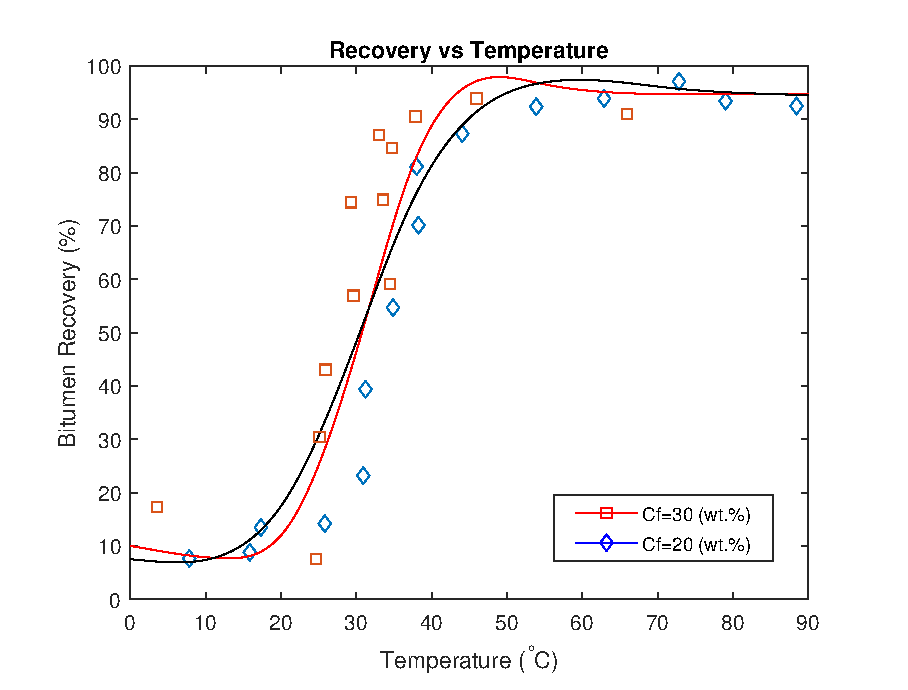
\includegraphics[width=\linewidth,clip]{T_comparison.eps}
	\vspace{-2em}
	\caption{Symbolic regression prediction of the relationship between recovery and temperature. Blue hollow square indicate actual data points. By altering clay fines amount to 30\%, red solid curve is visualized compared with original dark solid curve.}
	\label{t_comparison}
\end{figure}
\begin{figure}[!hptb]
	\centering
	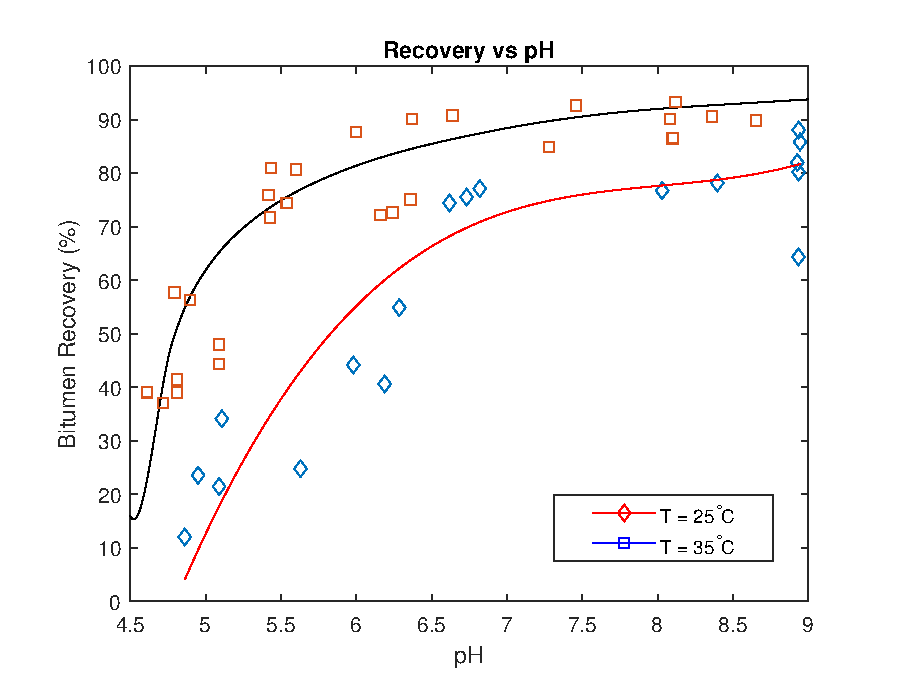
\includegraphics[width=\linewidth,clip]{ph_comparison.eps}
	\vspace{-2em}
	\caption{Symbolic regression prediction of the relationship between recovery and pH. Blue hollow square indicate actual data points. The difference between red and dark visualized curves is 10 degree alteration of temperature.}
	\label{ph_comparison}
\end{figure}

\begin{figure}[!hptb]
	\centering
	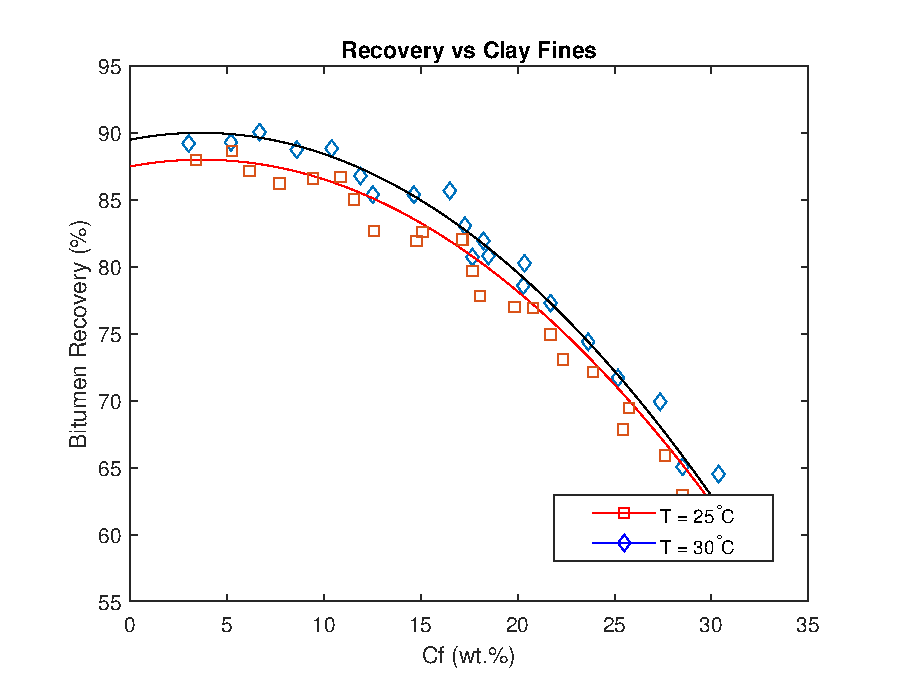
\includegraphics[width=\linewidth,clip]{Cf_comparison.eps}
	\vspace{-2em}
	\caption{Symbolic regression prediction of the relationship between recovery and clay fines. Blue hollow square indicate actual data points. The difference between red and dark visualized curves is 5 degree alteration of temperature. }
	\label{Cf_comparison}
\end{figure}


In \autoref{fig:sensitivity.eps}, the statistical performance of SR descriptor is further demonstrated, in which RMS errors between the SR result and the training and test dataset are compared respectively.

\begin{figure}[!hptb]
	\centering
	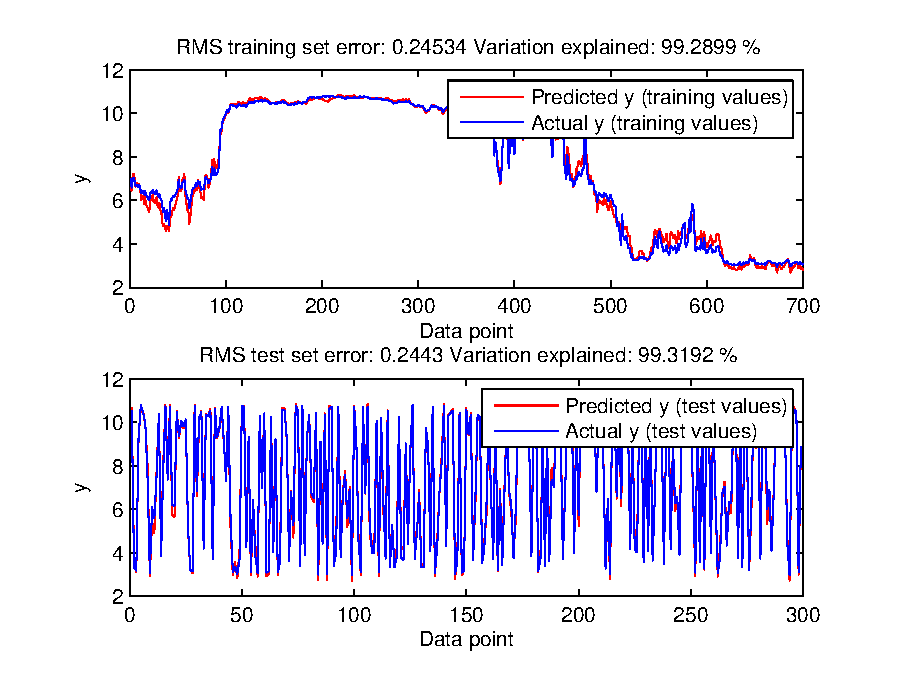
\includegraphics[width=\linewidth,clip]{sensitivity.eps}
	\vspace{-2em}
	\caption{Symbolic regression model performance.}
	\label{fig:sensitivity.eps}
\end{figure}


Finally, we evaluate the residuals between the observed value of the dependent variable and the predicted value (\autoref{fig:sensitivity2.eps}). Both the training and testing data indicate a non random patterns and show a good fit for the SR model.





\begin{figure}[!hptb]
	\centering
	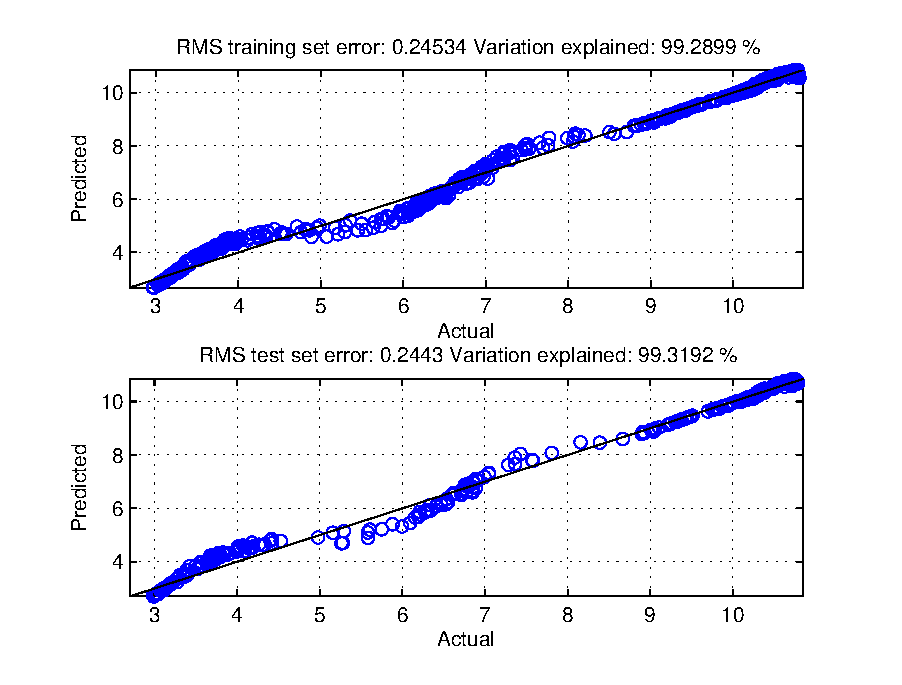
\includegraphics[width=\linewidth,clip]{sensitivity2.eps}
	\vspace{-2em}
	\caption{Symbolic regression prediction performance.}
	\label{fig:sensitivity2.eps}
\end{figure}





\section{Experimental Results of SR Descriptor} % (fold)
\label{sec:improvement}

\subsection{Data Description and Results}
The technology of near-infrared reflectance spectroscopy (NIRS) has been used for monitoring oil sands characteristics and operation procedure starting the 1950s.
Quantitative prediction of oil sands composition such as bitumen content, water content and magnesium concentration can be conducted using various models such as principal component regression (PCR), or artificial neural networks (ANN). The purpose of using NIRS data in oil sands analysis is to predict bitumen recovery. We will exhibit the SR descriptor using real world NIRS data in this section.

There are two probes for observing 9 measured variables: bitumen content, $Ca^{2+}$ concentration, Clays content, fines content, water content, $Mg^{2+}$ concentration, CL, Na and pH. At each probe there are 80000 data points. The NIRS data has been preprocessed for the purpose of converting spectrum data to numeric data.



% \begin{figure}[!hptb]	
% 	\captionsetup{labelformat=empty}
% 	\caption*{Table 2. Symbolic regression setup}.
% 	\centering
% 	\includegraphics[width=\linewidth]{table.png}
% 	\label{Table:setup}
% \end{figure}

\begin{table}[!hptb]
\centering
\caption*{Table 2. Symbolic regression setup}.
\label{my-label}
\begin{tabular}{|l|l|}
\hline
Setting               &                                \\ \hline
Population size       & 10000                          \\ \hline
Function set          & $+,-,x,/,sin,cos,tan,logistic$ \\ \hline
Fitness function      & RMSE                           \\ \hline
Selection method      & Tournament selection           \\ \hline
Crossover rate        & 90\%                           \\ \hline
Mutation rate         & 5\%                            \\ \hline
Number of generations & 2000                           \\ \hline
\end{tabular}
\end{table}

As shown in Table 2, for the SR program setup, we select the initial operator set ($+$, $-$, $\times$, $\div$) and the root mean square error (RMSE) as the fitness. The crossover rate is 90\%, indicating that more offspring can be generated. The mutation rate is 5\%.  

%Based on the given NIRS data, SR aims to extract an appropriate model from a space of all possible expressions $\mathcal{S}$ defined by a set of given binary operations (e.g., $+$, $-$, $\times$, $\div$, etc.) and mathematical functions (e.g., $\sin$, $\cos$, $\exp$, $\ln$, etc.), which can be described in the following nonlinear optimization problem:
% %\begin{equation}
% \label{SRdef}
% f^*=\arg\min_{f \in \mathcal{S}}\sum_i\left\|{f(\mathbf{x}^{(i)})-y_i}\right\|,
% %\end{equation}
% %where $\mathbf{x}^{(i)}\in{\mathbb{R}^d}$ and $y_i\in{\mathbb{R}}$ are input observations and output data, respectively. $f$ is the unknown target model and $f^*$ is the identified data model.

%\begin{table}[!hptb]
%	\centering
%	\footnotesize
%	\caption{GP settings.} 
%	 \setlength{\tabcolsep}{3pt}
%	\begin{tabular}{|l|c|c|}
%		\hline
%		\textbf{Setting}  &  \\
%		\hline
%		Population size	 & 200  \\
%		Function set         & 	{ $+$, $-$, $\times$, $\div$ }  \\
%		Fitness function	& Root mean squared error (RMSE)  \\
%		Initial population method & Ramped-half-and-half  \\
%		Selection method & Tournament selection  \\
%		Crossover rate & 90\%  \\
%		Mutation rate & 5\%  \\
%		Maximum tree depth in initial population & 6  \\
%		Number of generations & 100  \\
%		Number of runs & 50 independent runs for each test  \\                        
%		\hline		
%	\end{tabular}
%\end{table}

We conducted the SR via GP and obtained the following SR model after 1487 iterations.



%
%%\begin{align} 
%%\notag \bs R &= \frac{-0.00337}{Fines-5.79}  + logistic(0.0158 \cdot Fines^{-1} \cdot Bitumen)\\\notag
%%&\qquad + logistic(0.0147 \cdot Ca^{2+} \cdot Bitumen^{1.1})\\\notag
%%&\qquad + 0.00762 \cdot tanh(\frac{Bitmen \cdot Clays^{-1.798}}{Fines^{2.6} \cdot CL}) \\\notag
%%&\qquad - 0.00209 \cdot tanh(\frac{0.00186 \cdot Clays \cdot Bitumen}{logistic( 0.276 \cdot Fines \cdot Ca^{2+} }))\\\notag 
%%&\qquad + 0.0122 logistic ( CL \cdot Fines)\\\notag 
%%&\qquad + ...\\
%%\end{align}

\begin{align} \label{eq:NIRS}
\notag  R &= sin (\frac{0.069 \cdot Bitumen}{0.0746 - Fines})  + logistic(0.0739 \cdot Ca^{2+} \cdot Mg^{2+} )\\\notag
&\qquad - logistic(\frac{Na  \cdot Bitumen - Ca^{2+} }{0.0368 \cdot Mg^{2+}})\\\notag
&\qquad - 0.00137 \cdot tanh(H_2O \cdot CL - Fines^{-1} \cdot Na) \\\notag
&\qquad + logistic(\frac{Bitumen + 0.0239}{ Fines - 0.764 \cdot H_2O} )^2\\\notag 
&\qquad + ...\\
\end{align}

The above SR descriptor is obtained based on 8 input variables by removing the variable pH, because in the given NIRS dataset pH values do not vary much and are within a small range around certain constant.

Clearly the SR descriptor shown in \autoref{eq:NIRS} is different from the one obtained from the simulation data in Section 4. In this NIRS dataset, the pH value is very stable while in simulated dataset its values are assumed to be varying. Moreover, more input variables with respect to more oil sands characteristics are included, such as magnesium concentration and clays, hence the pattern in NIRS data will exhibit different characteristics in the model. 




\begin{figure}[!hptb]
	\centering
	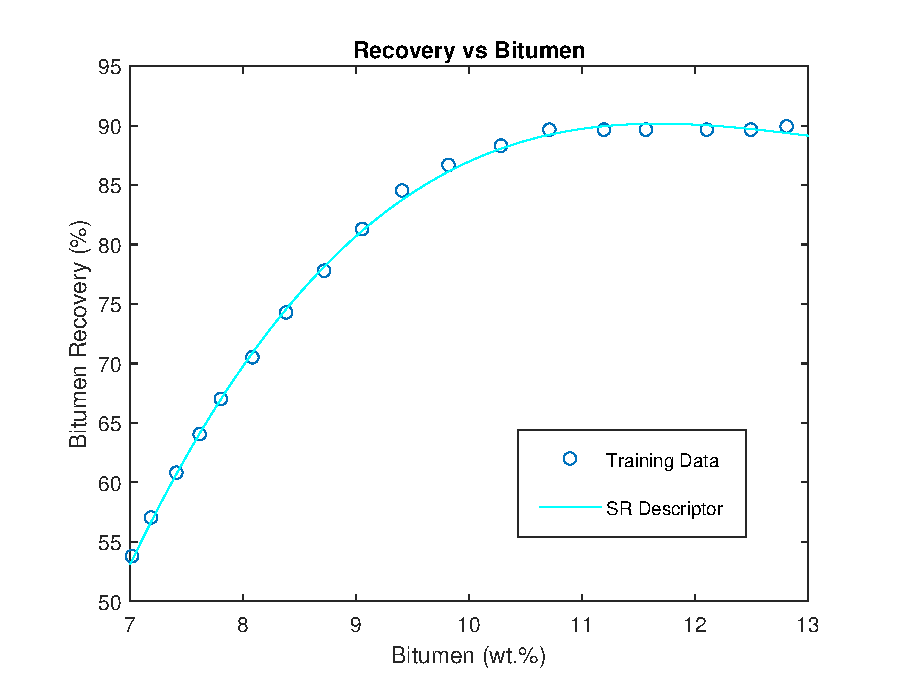
\includegraphics[width=\linewidth,clip]{NIRS_BITUMEN.eps}
	\caption{Symbolic regression prediction of the relationship between recovery and bitumen.}
	\label{fig:NIRS_BITUMEN}
\end{figure}


\begin{figure}[!hptb]
	\centering
	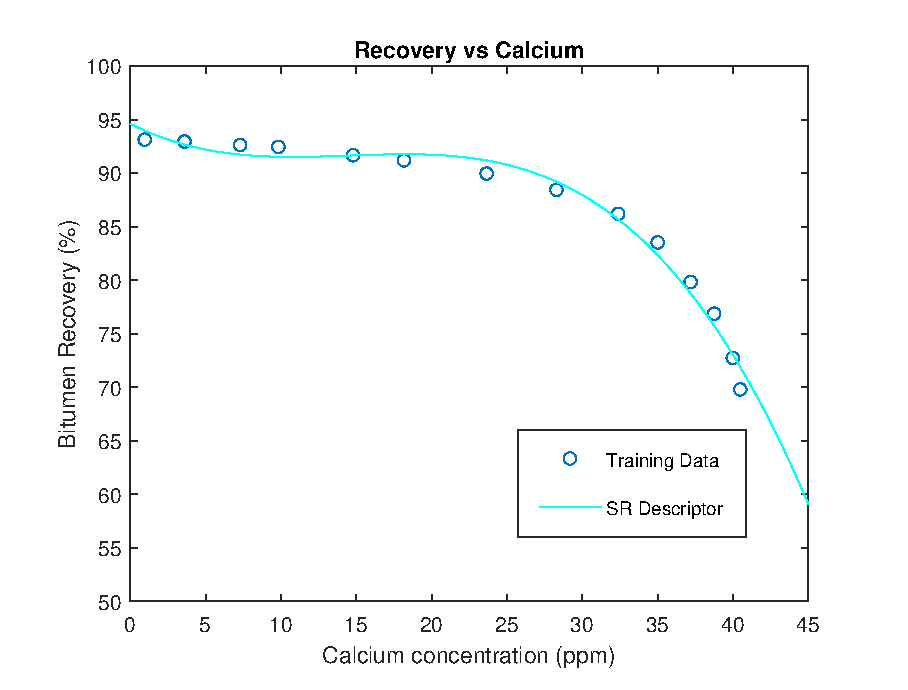
\includegraphics[width=\linewidth,clip]{NIRS_Calcium.eps}
	\caption{Symbolic regression prediction of the relationship between recovery and Calcium concentration.}
	\label{fig:NIRS_Calcium}
\end{figure}


\begin{figure}[!hptb]
	\centering
	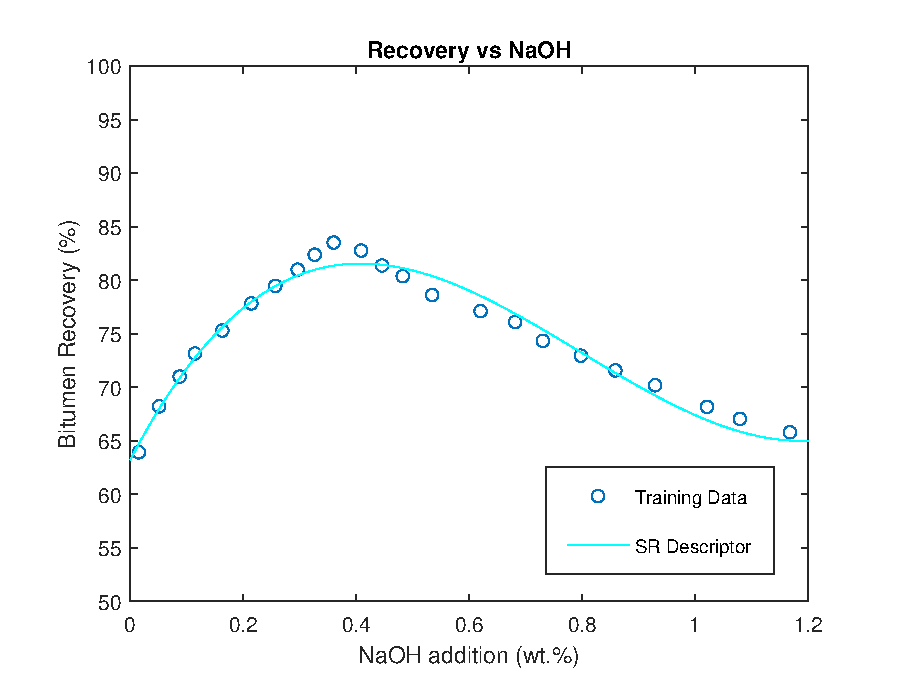
\includegraphics[width=\linewidth,clip]{NIRS_NaOH.eps}
	\caption{Symbolic regression prediction of the relationship between recovery and NaoH addition.}
	\label{fig:NIRS_NaOH}
\end{figure}

\begin{figure}[!hptb]
	\centering
	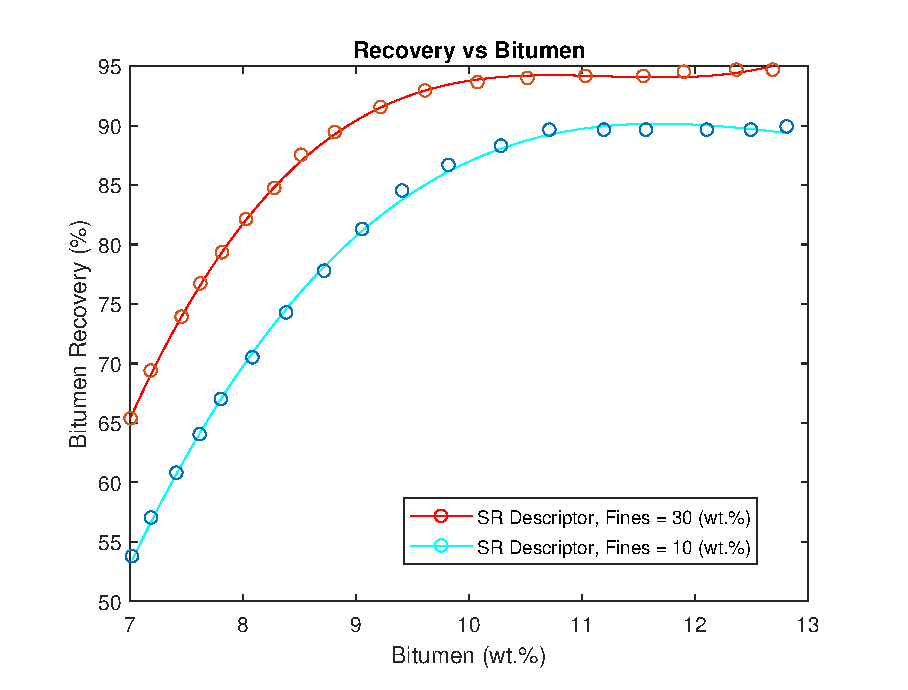
\includegraphics[width=\linewidth,clip]{NIRS_BITUMEN_COMPAIR.eps}
	\caption{Symbolic regression prediction of the relationship between recovery and bitumen content by different fines condition.}
	\label{fig:NIRS_BITUMEN_COMPAIR}
\end{figure}



%However, if we compare the model characteristics obtained for the fines variable in both simulation data and NIRS data, the results show show obvious similarities in their trends, as shown in \autoref{fig:CF_NIRS}.
%
%\begin{figure}[!hptb]
%	\centering
%	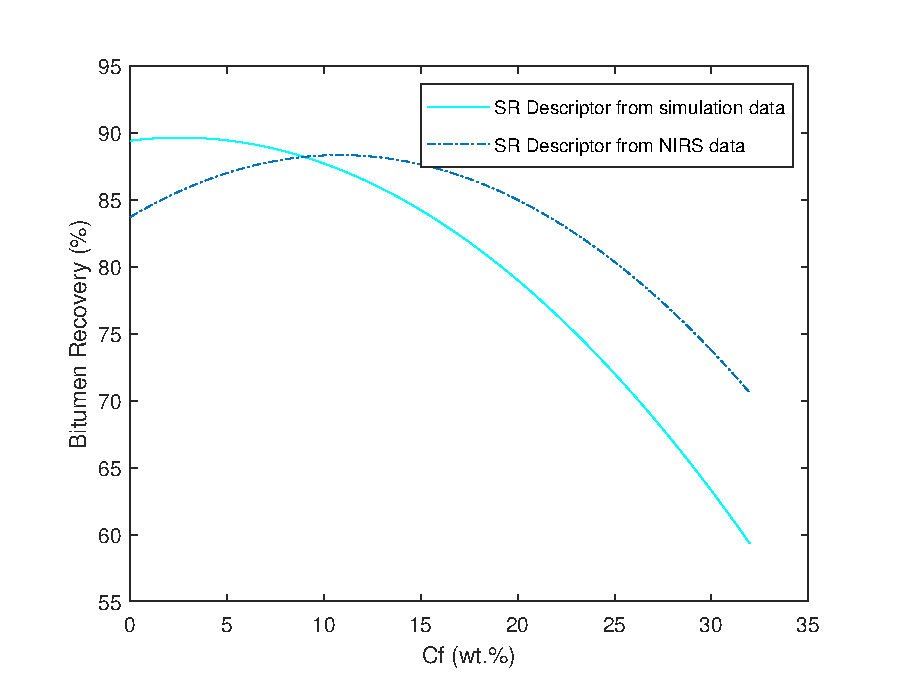
\includegraphics[width=\linewidth,clip]{CF_NIRS2.eps}
%    \caption{Symbolic regression model performance.}
%	\label{fig:CF_NIRS}
%\end{figure}
%
%
%
%%\begin{figure}[!hptb]	
%%	\captionsetup{labelformat=empty}
%%	\caption*{Table 3. Comparison of SR positive and negative sensitivity analysis}.
%%	\centering
%%	\includegraphics[width=\linewidth]{Magnitude.png}
%%	\label{Table:Magnitude_comparison}
%%\end{figure}
%
%The sensitivity analysis is performed to reveal relative importance of each input variable to the target variable (i.e. bitumen recovery), and the results are given in Table 2. 
%
%By \% Positive, it means the likelihood that increasing this variable will increase the target variable. If \% positive = 70\%, then for 70\% of total simulations increases in this variable lead to increases in the target variable (but for the remaining 30\% of the time it either decreases it or has no impact). If \% positive = 0\%, increases in this variable will not increase the target variable. When \% positive shows positive magnitude, this is generally how big the positive impact is.
%
%Similarly \% negative means the likelihood that increasing this variable will decrease the target variable. If \% negative = 60\%, then 60\% of the time increases in this variable lead to decreases in the target variable (but the remaining 40\% of the time it either increases it or has no impact). If \% negative = 0\%, increases in this variable will not decrease the target variable.
%
%In this analysis based on NIRS dataset, the SR descriptor shows that Clays is the most important indicator for bitumen recovery, and Bitumen content and CL are indicator having negative impact. For Fines and $Ca^{2+}$ concentration, the modeling results match the analysis from laboratory oil sands experiment.
%
%
%
\begin{figure}[!hptb]
	\centering
	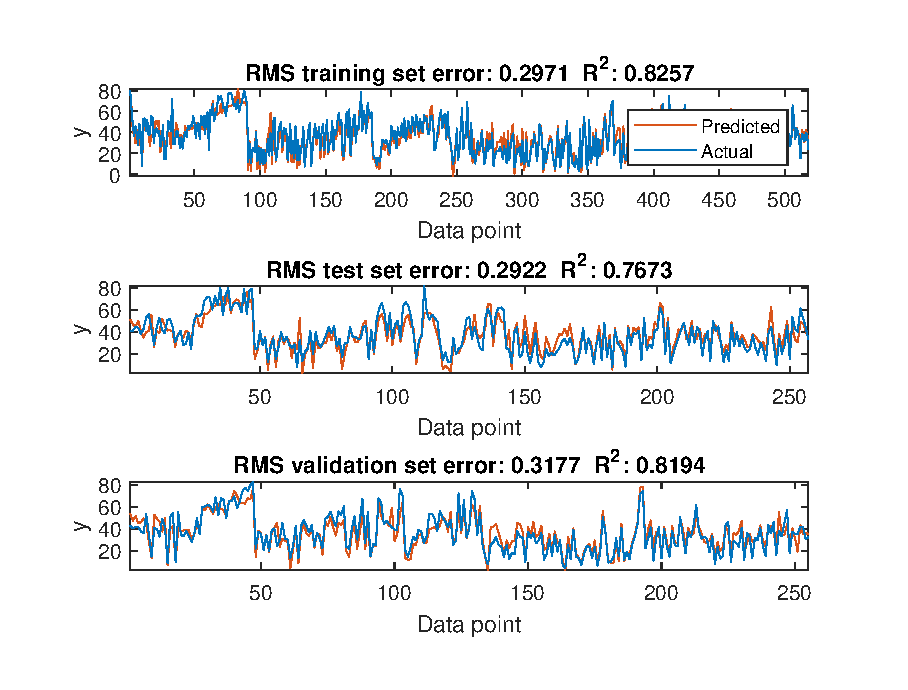
\includegraphics[width=\linewidth,clip]{NIR6.eps}
	
	\caption{Symbolic regression model performance.}
	\label{fig:NIR1}
\end{figure}
%
{\color{red} (You need to explain the new figures you added, e.g. Figure 11 -14 in the following paragraph...)}
The results showing relationship between several key variables and the bitumen recovery rate based on the SR descriptor are illustrated in \cref{fig:NIRS_BITUMEN,fig:NIRS_Calcium,fig:NIRS_NaOH}. Figures 11 - 13, respectively. In Figure 11, ...  In figure 12, .... 
.
To demonstrate the SR model prediction performance, \autoref{fig:NIR1} illustrates how actual recorded values compare with the predicted ones on both training and test datasets. In this study, we choose the training dataset size as 500, and both of the test data size and the validation dataset size as 250. We use k-fold (k=5) method on the validation dataset. Higher density of overlapping between the data points and the line exhibits better accuracy of the SR model. For fitness results, the RMS error is 0.2971 on training data set and 0.2922 on testing data set. On validation data set, the RMS error is slightly lower than that of both training and test data. In this study, we also calculate $R^2$, the coefficient used for sensitivity analysis. The $R^2$ value is 0.8194 in the validation data and 0.7673 in the test dataset.

\autoref{fig:NIR2} further shows the comparison between actual and predicted response. It shows a satisfactory match because the two responses align nicely along the diagonal line, which verifies the performance of the SR model. The vertical distance from the line to any point is the error of the prediction for that point. The RMS error is shown to be 0.3177 and $R^2$ error 0.8194, which are reasonably small. 

%\autoref{fig:NIR3} presents the residuals, which is the difference between the predicted and true responses. Positive values for the residual (on the y-axis) mean the prediction was too low, and negative values mean the prediction was too high. In our case, residuals have range from -0.5 to 1.%

\begin{figure}[!hptb]
	\centering
	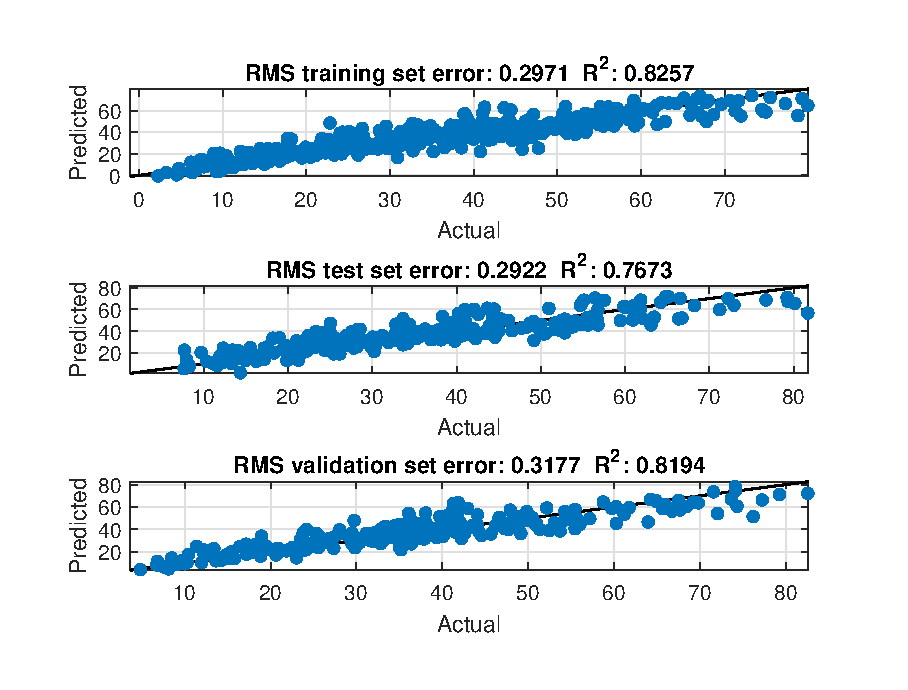
\includegraphics[width=\linewidth,clip]{NIR7.eps}
	
	\caption{Symbolic regression prediction response.}
	\label{fig:NIR2}
\end{figure}

%\begin{figure}[!hptb]
%	\centering
%	\includegraphics[scale=.35]{NIR3.png}
%
%	\caption{Symbolic regression residual.}
%	\label{fig:NIR3}
%\end{figure}

%
%
%

\subsection{Discussions}

\noindent
\textbf{Remark 1} Physical Knowledge vs Model Accuracy

It is noted that there exists a trade-off between making prediction based on data and analysis based on physical knowledge. In many cases, knowledge about the process can help improve the model by providing meaningful physical interpretation. However a key question is how to take advantage of physical knowledge. For example, in oil sands research, theoretical knowledge regarding bitumen recovery and processability of oil sands ores exist, but there still exist many uncertainties and unknown characteristics. Researchers rely on experimental data in this case.
....
In this experiment, we compare results from SR model from different perspective which means prior knowledge is involved. Common facts from bitumen recovery processability can be hand-crafted into SR model as iteration blockers.
For example, fines content has negative impact on bitumen recovery compared with bitumen content. Water content also has negative correlation with bitumen recovery. With those prior human knowledge, the following selected function sets :${B/F}$,${1/Ca^2+}$ have been structured as blockers.

Again, the ability of SR model to learn from experience means it can learn from experience: given enough experiment results regarding how to process bitumen, such as more oil sands characteristics and operation conditions, SR model can learn from this process and make accurate predictions.

We presented two results: $R_1$ without prior knowledge and $R_2$ with setup features.

\begin{align*} 
    \notag R_1 &= \frac{-0.00337}{Fines-5.79}  + logistic(0.0158 \cdot Fines^{-1} \cdot Na)\\\notag
    &\qquad + logistic(0.0147 \cdot Ca^{2+} \cdot Bitumen^{1.1})\\\notag
    &\qquad + 0.00762 \cdot tanh(\frac{Bitmen \cdot Clays^{-1.798}}{Fines^{2.6} \cdot CL}) \\\notag
    &\qquad - 0.00209 \cdot tanh(\frac{0.00186 \cdot Mg^2+ \cdot Bitumen}{logistic( 0.276 \cdot Fines \cdot Ca^{2+} }))\\\notag 
    &\qquad + 0.0122 logistic ( CL \cdot H_2O)\\\notag 
    &\qquad + ...\\
\end{align*}



\begin{align} 
    \notag R_2 &= sin (\frac{0.069 \cdot Bitumen}{0.0746 - Fines})  + logistic(0.0739 \cdot Ca^{2+} \cdot Mg^{2+} )\\\notag
    &\qquad - logistic(\frac{Na  \cdot Bitumen - Ca^{2+} }{0.0368 \cdot Mg^{2+}})\\\notag
    &\qquad - 0.00137 \cdot tanh(H_2O \cdot CL - Fines^{-1} \cdot Na) \\\notag
    &\qquad + logistic(\frac{Bitumen + 0.0239}{ Fines - 0.764 \cdot H_2O} )^2\\\notag 
    &\qquad + ...\\
\end{align}

\autoref{fig:R1vsR2} shows the comparison between $R_1$ and $R_2$ results on bitumen contents. This comparison is purely for our objective reagaring statistically improvement. With prior knowledge, oil sands characteristics has been transformed into features that crafted into SR model. Moreover, SR model has been improved as a physical guideline for bitumen recovery processability. 

\begin{figure}[!hptb]
	\centering
	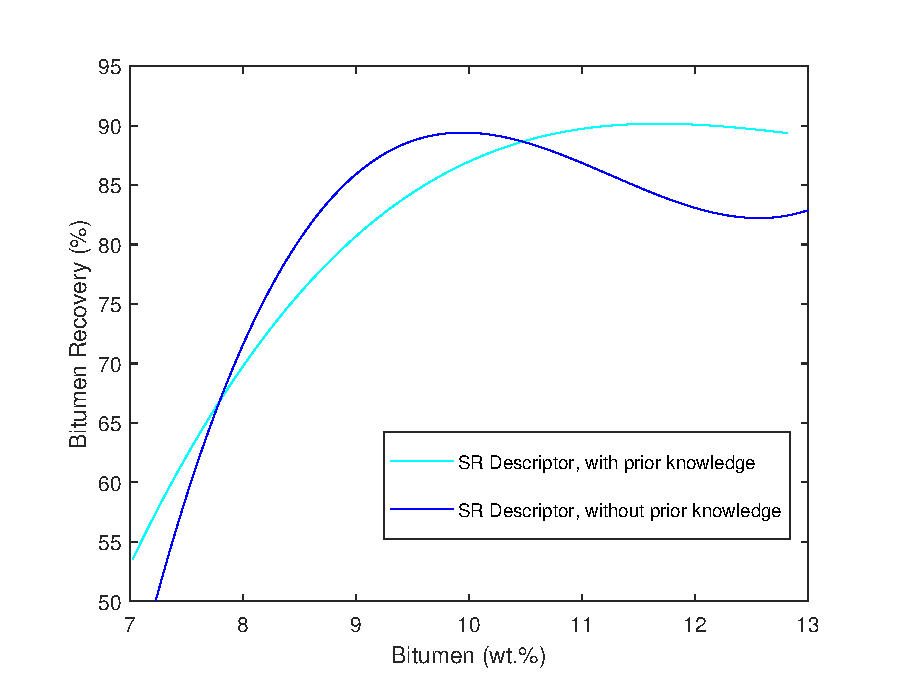
\includegraphics[width=\linewidth,clip]{R1VSR2.eps}
	\caption{Symbolic regression prediction results with prior knowledge.}
	\label{fig:R1vsR2}
\end{figure}

\noindent
\textbf{Remark 2} Hybrid modeling

The advantage of this hybrid approach is that we can perform our data-driven model the physics of the problem by generating large amounts of training data from bitumen processability. The hybrid modeling methodology can be addressed in the algorithmic approach. 

For traditional analytical modeling, basic rules or experiences only target a domain-specific formulation. Physical experiments are designed meticulously, intending with less human errors. However, there are may remaining modeling errors, for example due to lack of suitable models, or imprecise knowledge of extrapolation.

On the contrary, data-driven modeling such as symbolic regression approach can make an improvement of accuracy and most often address universal function approximators. In this process, feature selection of the training data, algorithm design and complexity are required.

We boldly propose a hybrid model that is a combination of parametrized analytical physical model with a data-driven model. The hybrid model requires a domain-specific model and also a data-driven model for the purpose of approximations. The results will have a gray-box characteristic combining explicit knowledge with a data-driven approach, which leaves a open discussion \autoref{fig:hybrid}.

\begin{figure}[!hptb]
	\centering
	\includegraphics[width=0.5\textwidth]{hybrid.png}
	\caption{A overview of hybrid modeling.}
	\label{fig:hybrid}
\end{figure}


\section{Conclusion} % (fold)
\label{sec:conclusion}
We have introduced a novel symbolic regression model for oil sands recovery prediction, which is capable of selecting an optimum combination of function candidates and a set of mathematical operators so that the data can be described by the constructed mathematical descriptor. Furthermore, we show that the proposed technique is able to understand a combination of representations for oil sands recovery with respect to the sensible markers obtained using a simulation oil sands data and real world data set.

One important future work is to improve our experimental results and further interpretation for the industrial plant data.


\section*{Acknowledgments}

This study was funded through Natural Sciences and Engineering Research Council of Canada (NSERC). 

%% References
%%
%% Following citation commands can be used in the body text:
%% Usage of \cite is as follows:
%%   \cite{key}         ==>>  [#]
%%   \cite[chap. 2]{key} ==>> [#, chap. 2]
%%

%% References with bibTeX database:

%\bibliographystyle{elsarticle-num}
\bibliographystyle{elsarticle-harv}
%\bibliographystyle{elsarticle-num-names}
% \bibliographystyle{model1a-num-names}
% \bibliographystyle{model1b-num-names}
% \bibliographystyle{model1c-num-names}
% \bibliographystyle{model1-num-names}
% \bibliographystyle{model2-names}
% \bibliographystyle{model3a-num-names}
% \bibliographystyle{model3-num-names}
% \bibliographystyle{model4-names}
% \bibliographystyle{model5-names}
% \bibliographystyle{model6-num-names}

\bibliography{sample.bib}

\cleardoublepage

\appendix 

\section{}
\begin{figure*}
	\centering
	\includegraphics[width=0.2\textwidth]{C.png}
	\caption{Flowchart of symbolic regression algorithm.}
	\label{fig:AF}
\end{figure*}


\end{document}

%%
%% End of file `elsarticle-template-num.tex'.
